\cotefile{123}
\scanpage{22}
\handwritten{\unsure{Massy} 22. 10. 1969}\\

Dear Kostant,\\

I read again through your papers in the \unsure{Maer.|Amer.} Journ. on \handwritten{``}\deleted{t}\handwritten{T}he principal three-dimensional subgroup ...\handwritten{''} and \handwritten{``}Lie group representations on polynom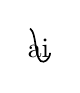
\begin{tikzpicture}[baseline=(letters.base),x=1em,y=1em]
\node[inner sep=0pt] (letters) at (0,0) {ai};
\handwritten{\draw[line width=.6pt] (-.30,.72) .. controls (-.04,.55) and (-.16,-.55) .. (.19,-.48) .. controls (.34,-.46) and (.44,-.22) .. (.42,-.16);}
\end{tikzpicture}l rings\handwritten{''}, prompted by some nice work of Brieskorn on Klein singularities. I very much appreciate this work of yours, and would appreciate getting reprints of any later work you may have available. As I already felt when your work appea\unsure{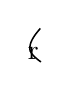
\begin{tikzpicture}[baseline=(r.base),x=1em,y=1em]
\node[inner sep=0pt] (r) at (0,0) {r};
\handwritten{\draw[line width=.55pt] (.25,.92) .. controls (.02,.66) and (-.18,.38) .. (-.12,.11) .. controls (-.07,-.03) and (.14,-.20) .. (.27,-.29);}
\end{tikzpicture}|k}ed, it cries for careful reconsideration in the framework of \deleted{\unsure{a|A}}\handwritten{A}lg. Geometry, and suggests number of interesting problems. I wonder if you know the answer to some of them. For instance, I feel it would be of interest to classify (for a given complex simple adjoint Lie group, say) quadr\deleted{\unsure{a|u}}uples $(\mathrm{T},\mathrm{B},\mathrm{T}',\mathrm{B}')$, where $\mathrm{T}$ and $\mathrm{T}'$ are maximal tori ``in apposition\handwritten{''} (in your terminology), and $\mathrm{B}$ and $\mathrm{B}'$ Borel subgroups of $\mathrm{G}$ containing $\mathrm{T}$ resp. $\mathrm{T}'$. The number of conjugacy classes of such animals is equal to $\operatorname{card}(\mathrm{W})^{\handwritten{2}}/\mathrm{hz}\handwritten{\phi}(\mathrm{h})$, where $\deleted{\unsure{\mathrm{H}|\mathrm{W}}}\handwritten{W}$ is the Weyl group, $\mathrm{h}$ the Coxeter number, $\mathrm{z}$ the order of the 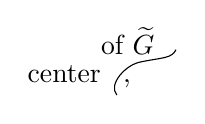
\begin{tikzpicture}[baseline=(center.base),x=1em,y=1em]
\node[anchor=base west,inner sep=0pt] (center) at (0,0) {center};
\node[anchor=base west,inner sep=0pt] at (3.45,0) {,};
\node[anchor=base west,inner sep=0pt] at (2.65,1.02) {\inserted{\handwritten{of $\widetilde{G}$}}};
\handwritten{\draw[line width=.4pt] (3.24,-.44) .. controls (2.91,-.05) and (3.58,.68) .. (4.12,.76) .. controls (4.89,.92) and (5.23,.88) .. (5.38,1.20);}
\end{tikzpicture} and $\handwritten{\phi}(\mathrm{h})=\operatorname{card}(\underline{\mathrm{Z}}/\mathrm{h}\underline{\mathrm{Z}})^{\handwritten{*}}$ is the Euler indicatrix; if you want to classify such data with moreover a\deleted{n} 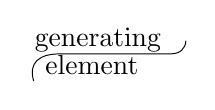
\begin{tikzpicture}[baseline=(element.base),x=1em,y=1em]
\node[anchor=base west,inner sep=0pt] (element) at (0,0) {element};
\node[anchor=base west,inner sep=0pt] at (-.38,1.04) {\inserted{generating}};
\handwritten{\draw[line width=.35pt] (-.40,-.22) .. controls (-.60,.44) and (-.20,.75) .. (.50,.76) -- (4.55,.76) .. controls (4.91,.77) and (5.08,.95) .. (5.10,1.24);}
\end{tikzpicture} (principal regular in your terminology) given for the finite group of order $\mathrm{h}$ $\mathrm{T}\handwritten{\cap}\mathrm{N}(\mathrm{T}')$, then we get $\operatorname{card}(\mathrm{W})^{\handwritten{2}}/\mathrm{hz}$ choices. One of the reasons I think this question is interesting is that the stablity subgroup in $\mathrm{G}$ of such a quadruple is $\mathrm{T}\handwritten{\cap}\mathrm{T}'=\mathrm{e}$,\handwritten{\textsuperscript{*}} hence such a structure makes $\mathrm{G}$ entirely ``rigid'' up to exterior automorphisms. Among the first questions one may wish to ask in this direction are the following: is it true that for some, or for all, such quadruples, $\mathrm{B}$ and $\mathrm{B}'$ are ``in general position'' i.e. $\mathrm{B}\handwritten{\cap}\mathrm{B}'$ is a torus (necessarily maximal), so that $\mathrm{B}$ and $\mathrm{B}'$ are ``opposite'' to each other with respect to the latter ? Is there in any sense a \uline{distinguished} conjugacy class of such quadruples (which should then be, of course, invariant by action of exterior automorphisms) ? What are the groups of automorph\unsure{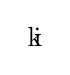
\begin{tikzpicture}[baseline=(k.base),x=1em,y=1em]
\node[inner sep=0pt] (k) at (0,0) {k};
\node[inner sep=0pt] at (.10,0) {i};
\end{tikzpicture}}sms of such quadr\deleted{a}uples (they


\margin{\handwritten{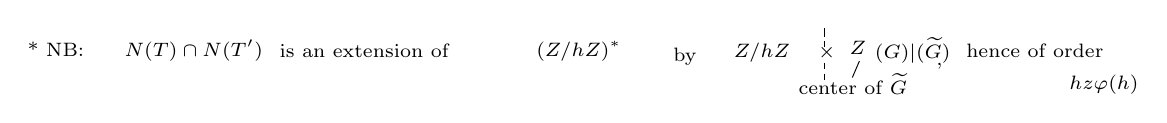
\begin{tikzpicture}[x=1cm,y=1cm,every node/.style={inner sep=0pt,anchor=base west,font=\scriptsize}]
\node at (0,0) {* NB:};
\node at (1.23,0) {$N(T)\cap N(T')$};
\node at (3.20,-.02) {is an exten\unsure{s}ion of};
\node at (6.46,0) {$(\mathbb{Z}/h\mathbb{Z})^{*}$};
\node at (8.20,-.06) {by};
\node at (8.97,-.02) {$\mathbb{Z}/h\mathbb{Z}$};
\node at (10.04,-.02) {$\times$};
\draw[line width=.2pt] (10.13,.36)--(10.13,.25) (10.13,.19)--(10.13,.12) (10.13,-.08)--(10.13,-.16) (10.13,-.22)--(10.13,-.30);
\node at (10.44,.02) {$Z$};
\node at (10.76,-.03) {$\deleted{\unsure{(G)|(\widetilde{G})}}$};
\node at (11.54,-.12) {,};
\draw[line width=.35pt] (10.57,-.06)--(10.48,-.27);
\node at (9.79,-.49) {center of $\widetilde{G}$};
\node at (11.92,-.02) {hen\unsure{ce} of order};
\node at (13.23,-.42) {$hz\varphi(h)$};
\end{tikzpicture}}}
% Bottom margin note: the final order is on a lower row at the right;
% the annotation center of G-tilde is below and left of the live Z.
% The separate interrupted vertical trace through the multiplication sign is reproduced without assigning it a mathematical function.
% The pen trace through the r/k cell in appeared and the typewriter k/i overprint in automorphisms do not securely establish correction chronology.
% The handwritten transposition stroke crosses the original typed ai in polynomail; no replacement letters have been supplied.
% archive sheet number: 21
